\chapter{Pasi necesari pentru a reproduce}

Informatii despre replicarea conditiilor necesare executiei programelor scrise folosind F* se pot gasi pe pagina de github a limbajului F*. \footnote{https://github.com/FStarLang/FStar/blob/master/INSTALL.md}

In sectiunea urmatoare se prezinta pasii care au fost luati pentru crearea mediului in care s-a dezvoltat 'SAT solver-ul'. Instructiunile urmatoare sunt compatibile cu sistemul de operare Windows, verificat cu versiunile 10/11. 

\section{Programe si resurse necesare}

Urmatoarele aplicatii/programe/resurse trebuie descarcate de la locatia specificata fiecareia in fisierul 'INSTALL.md' gasit pe pagina de github a limbajului FStar.

\begin{itemize}
 \item OCaml - necesar compilarii si executarii fisierelor OCaml (.ml), care rezulta in urma compilarii fisierelor FStar (.fst)
	
 \item opam - necesar pentru a instala pachetele necesare la compilarea fisierelor specifice limbajului de programare OCaml (versiune folosita - 4.14.0)
 
 (versiunea folosita pentru lucrare - 2.0.10)
 \item cygwin - ofera posibilitatea compilarii si executarii a programelor tipice sistemelor de operare Unix si Linux, ceea ce include suport pentru fisiere 'Makefile' 
 
 (versiunea folosita pentru lucrare - 3.4.6)
 \item Z3 - folosit pentru a valida fisierele ce contin programe scrise folosind F*
 

 
 (arhiva folosita pentru Windows - z3-4.8.5-x64-win.zip)
\end{itemize}

\newpage


Dupa descarcarea/instalarea acestor resurse, trebuie clonata ramura 'master' a proiectului FStar pe dispozitivul local, denumind folder-ul "fstar". (locatia clonei pentru acest proiect: "D:/fstar", versiunea  - F* 2023.04.26~dev )

Trebuie adaugate path-urile absolute catre ".../fstar/bin" si ".../z3-win/bin" in variabila 'Path' a sistemului.

Dupa instalarea programului 'opam', trebuie instalate mai anumite pachete de date. Minimul necesar de pachete se poate gasi si pe instructiunile de instalare gasite la link-ul de mai sus, insa pentru a avea la dispozitie toate resursele din proiectul FStar descarcat fara erori, sunt necesare urmatoarele pachete: 
\newline

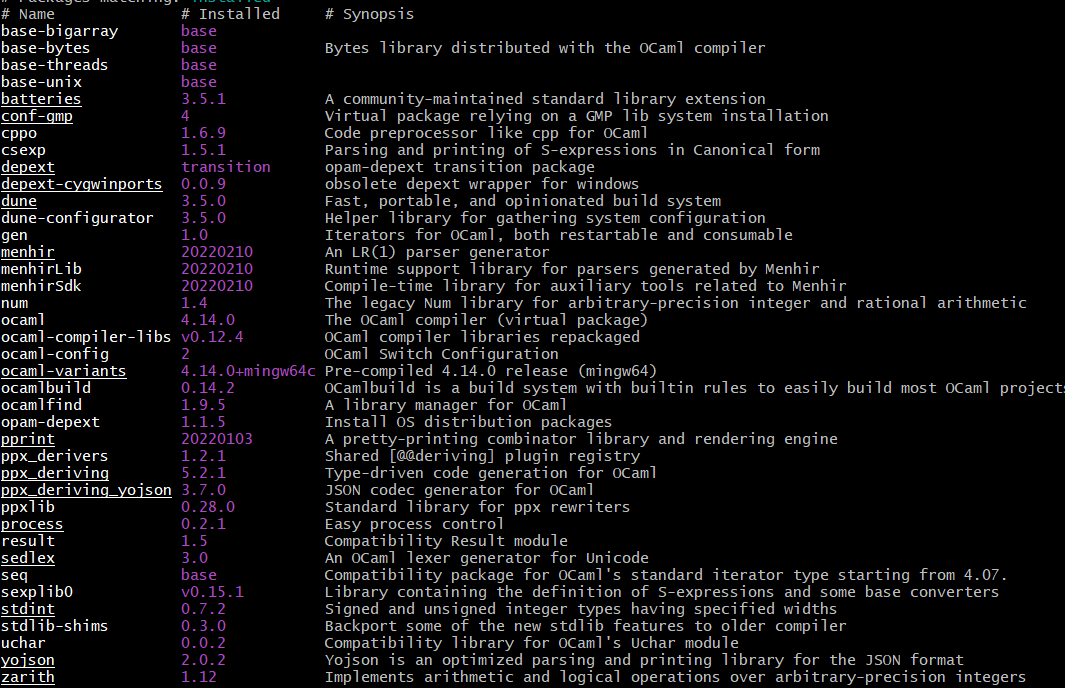
\includegraphics[width=1\textwidth]{opam_necesary_packages.png}
\newline

La finalul acestor pasi, folosind terminalul Cygwin si instructiunile de tipul 'make' in folder-ul 'fstar', ar trebui sa functioneze verificarea si executarea oricaror fisiere surse scrise in F*, fisiere proprii sau exemple ce faceau deja parte din proiect.

\newpage

\section{Executarea solver-ului SAT}

Sursele corespunzatoare proiectului prezentat se gasesc la:
\href{https://github.com/alex4482/FStar-DPLL-licenta/tree/main/dpll_optimized}{FStar-DPLL github}.

Aceste surse trebuie descarcate, salvate intr-un folder in proiectul 'fstar'. Fisierul 'Makefile' trebuie modificat, astfel incat variabila 'FSTAR-HOME' trebuie sa faca referire folder-ul 'fstar'. Aceiasi pasi trebuie facuti pentru fisieru 'Makefile' din folder-ul 'output'.

Apoi, in terminalul cygwin deschis in folder-ul proiectului DPLL-FStar, trebuie executata comanda 'make', la finalul careia in folder-ul 'output' vor aparea pentru fiecare fisier sursa '.fst' cate un fisier '.ml' care contin codul Ocaml extras din sursele FStar. De asemenea in folder-ul 'output' se va afla executabilul "Main.exe".

Pentru a recompila si regenera fisierul "Main.exe", trebuie sters cel anterior creat, daca a fost creat.

Imediat dupa pornirea programului "Main.exe", trebuie introdus de la tastatura calea relativa catre un fisier de input. Cateva fisiere de input exista in folder-ul "input-files" si orice alt fisier de intrare trebuie sa respecte acel pentru ca parsarea implementata a datelor sa functioneze.

La finalul unei astfel de executii, va aparea mesaj la consola cygwin cu rezultatul obtinut, fie ca formula data este nesatisfiabila, fie ca e satisfiabila si alaturi o varianta de raspuns ce contine variabilele formulei si valorile lor astfel incat fiecare clauza a formulei sa aibe valoarea de adevar true.

-----INTRODU EXEMPLU POZA INPUT / OUTPUT DUPA EXECUTIE
